\documentclass{scrartcl}
\usepackage[utf8]{inputenc}
\usepackage{amsmath}
\usepackage{graphicx}
\usepackage{tabularx}
\usepackage{amssymb}
\usepackage{hyperref}
\renewcommand{\contentsname}{Inhaltsverzeichnis}
\begin{document}
\title{\Huge{YUV.KA} \\ \large{Praxis der Softwareentwicklung 2011/2012}}
\author{Max Wagner $\cdot$ Patrick Gemander $\cdot$ Sebastian Ullrich $\cdot$ Michael Vollmer \\ Robert Hangu $\cdot$ Daniel Lebert}
\maketitle

\newpage
\mbox{}

\addcontentsline{toc}{section}{Inhaltsverzeichnis}
\tableofcontents
\section{Einleitung}

Es soll ein Multimedia-Framework zur Evaluation von Videoencodern erstellt werden. Hierzu sollen Videos erzeugt und verändert werden können. Diese sollen anschließend von einem Videoencoder encodiert werden. Des Weiteren sollen die erzeugten Videos mit Referenzvideos verglichen werden, um eventuelle Schwächen des Encoders aufzuzeigen. In diese Analyse sollen auch Informationen der Encoder einfließen.

\section{Zielbestimmung}

Die Firma soll durch das Produkt in die Lage versetzt werden, Encoder zu testen, indem encodierte Videos manipuliert und anhand eines Referenzvideos verglichen werden.

\subsection{Musskriterien}

\begin{itemize}
	\item Eingabe von (encodierten) Videos, einer festen Farbe, einem Bild oder Noise
	\item Manipulation der Videos
	\begin{itemize}
		\item Erstellen einer Pipeline mit verschiedenen Manipulationsoptionen
		\item Zusammenstellung über knotenbasierte GraphView
	\end{itemize}
	\item Analyse der Videos
	\begin{itemize}
		\item Anzeigen verschiedener Diagramme
		\item Videoausgabe mit optionalen Overlayoptionen
	\end{itemize}
	\item Speichern der Videos und Pipeline
\end{itemize}

\subsection{Wunschkriterien}

\begin{itemize}
	\item Undo/Redo-Funktion
	\item Interface mit Tabs
	\item Automatische Resolution-Erkennung
	\item Asynchrone, nichtblockende UI
	\item Multithreading
	\item Kommandozeilenversion
\end{itemize}

\subsection{Abgrenzungskriterien}

\begin{itemize}
	\item keine Soundausgabe
	\item nur YUV-Videos als Eingabe
	\item keine Speicherung der Analysedaten
\end{itemize}

\section{Produkteinsatz}

Das Produkt dient zum Testen der eigens entwickelten Encoder bzw. deren Videos.

\subsection{Anwendungsbereiche}

Manipulation und Analyse von Videos (professioneller Anwendungsbereich)

\subsection{Zielgruppen}

Die Zielgruppe sind Entwickler des zu testenden Encoders, sodass ein gewisses Vorwissen über Videomanipulation vorrausgesetzt werden kann.

\subsection{Betriebsbedingungen}

Einsatz in der Entwurfsumgebung, in der auch die Encoder entwickelt wurden.

\section{Produktumgebung}

\begin{itemize}
	\item Windows 7 oder neuer
	\item .NET Framework 4.0 oder neuer
\end{itemize}

\section{Funktionale Anforderungen}

\subparagraph{Input/Output zur Videobearbeitung} 
\begin{itemize} 
	\item \textbf{/F10/} Einlesen eines Videos im yuv-Format.
	\item \textbf{/F20/} Erzeugung von (Perlin-)Noise.
	\item \textbf{/F30/} Einlesen einer Bilddatei als Standbild-Video.
	\item \textbf{/F40/} Speichern eines Videos als yuv-Datei.
	\item \textbf{/F50/} Speichern und Laden der erstellten Bearbeitungs-/Analysepipelines
	\item \textbf{/F60/} Konstante Farbe als Standbild-Video.
\end{itemize}

\subparagraph{Videobearbeitung}
\begin{itemize}
	\item \textbf{/F100/} Trennung nach den RGB-Farbkanälen.
	\item \textbf{/F110/} Additives Übereinanderlegen mehrerer Videos.
	\item \textbf{/F120/} Gewichtet gemitteltes Übereinanderlegen mehrerer Videos.
	\item \textbf{/F130/} Lineares und Gauß'sches Weichzeichnen von Videos.
	\item \textbf{/F140/} Farbinvertierung eines Videos.
	\item \textbf{/F150/} Quantisieren der Farbpalette eines Videos.
	\item \textbf{/F160/} Änderung von Kontrast, Farbsättigung und Helligkeit eines Videos.
	\item \textbf{/F170/} Verzögern eines Videos um $n$ Frames.	
	\item \textfb{/F180/} Bilden des Differenzvideos zweier Videos.
\end{itemize}

\subparagraph{Videoanalyse}
\begin{itemize}
	\item Analyse eines einzelnen Videos  
		\begin{itemize}
			\item \textbf{/F200/} Anzeigen der I/P/B-Frames eines Videos.
			\item \textbf{/F210/} Anzeigen des Helligkeitsverlaufs eines Videos pro Frame.
			\item \textbf{/F230/} Anzeigen des Histogramms eines Video.
			\item \textbf{/F240/} Anzeigen der Pseudo-Noies-Ratio pro Frame.
		   \end{itemize} 
	\item Vergleich eines oder mehrerer Videos mit einem Referenzvideo
		\begin{itemize}
			\item \textbf{/F300/} Differenz der Pixelfarben.
			\item \textbf{/F310/} Differenz der Encoder-Entscheidungen.
			\item \textbf{/F320/} Anzahl der Artefakte.
			\item \textbf{/F330/} Videoansicht mit Highlighting der Artefakte.
		\end{itemize}	
	\item Sonstiges
		\begin{itemize}
			\item \textbf{/F400/} Anzeigen eines Videos. 
			\item \textbf{/F410/} Die Punkte /F10/ bis /F330/ sollen im Rahmen der Rechnerleistung beliebig kombinierbar sein.
		\end{itemize}
\end{itemize}


\section{Produktdaten}

\begin{itemize}
	\item \textbf{/PD10/} YUV-Videodateien und ggf. dazugehörige Logdateien als Input
	\item \textbf{/PD20/} Standbilder als Input
	\item \textbf{/PD30/} Gespeicherte Pipelines
\end{itemize}

\section{Systemmodell}

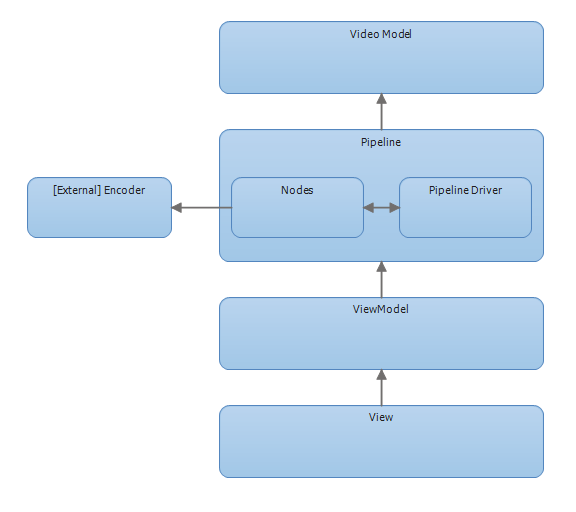
\includegraphics[scale=0.75]{resources/Layers}

\section{Entwicklungsumgebung}

\begin{itemize}
	\item Windows 7
	\item Visual Studio 2010 Ultimate + Expression Blend 4
	\item WPF Toolkit
	\item Git for Windows
	\item Dual- bis QuadCore
\end{itemize}

\section{Produktleistungen}

\subparagraph{Benutzbarkeit}
\begin{itemize}
	\item \textbf{/L10/} Die Benutzeroberfläche soll einfach und intuitiv zu bedienen sein. Unerfahrene Benutzer sollen ohne Vorwissen in der Lage sein, sich schnell in die Funktionalitäten einzuarbeiten.
	\item \textbf{/L20/} Die Zusammenstellung sowie die Nacheinanderreihung der verschiedenen Manipulationseffekte soll einfach und übersichtlich geschehen können. 
	\item \textbf{/L30/} Der Benutzer muss in der Lage sein, neue Manipulationseffekte hinzuzufügen, ohne die Reihenfolge der bereits bestehenden ändern zu müssen.
	\item \textbf{/L40/} Im Programm sollen theoretisch gleichzeitig uneingeschränkt viele Videos verwaltet, bearbeitet und analysiert werden können.
	\item \textbf{/L50/} Der Benutzer muss ein Video aus jeder Stufe der Bearbeitung problemlos abspielen, analysieren oder exportieren können.
\end{itemize}

\subparagraph{Geschwindigkeit}

\begin{itemize}
	\item \textbf{/L100/} Bei einer einfachen analysefähigen Pipeline mit einem einzigen Manipulationseffekt sollen ein Video der Auflösung 320p und die zugehörigen Statistiken in Echtzeit ausgegeben werden können.
\end{itemize}

\subparagraph{Robustheit}

\begin{itemize}
	\item \textbf{/L200/} Das Programm soll trotz falscher Benutzereingaben oder Parameter nicht abstürzen. Es muss in diesen Fällen entsprechend reagieren.
\end{itemize}

\subparagraph{Erweiterbarkeit}

\begin{itemize}
	\item \textbf{/L300/} Das Programm soll sich einfach um neue Funktionalitäten erweitern lassen.
\end{itemize}

 

\section{Bedienoberfläche}

\begin{figure}[h!]
	\centering
	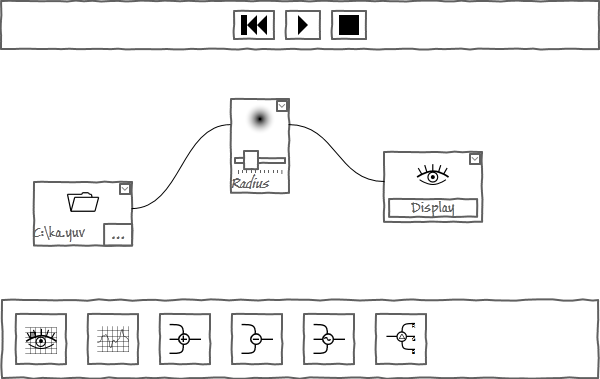
\includegraphics[scale=0.8]{resources/main-screen.png}
	\caption{Hauptoberfläche des Programms}
\end{figure}
\begin{figure}[h!]
	\centering
	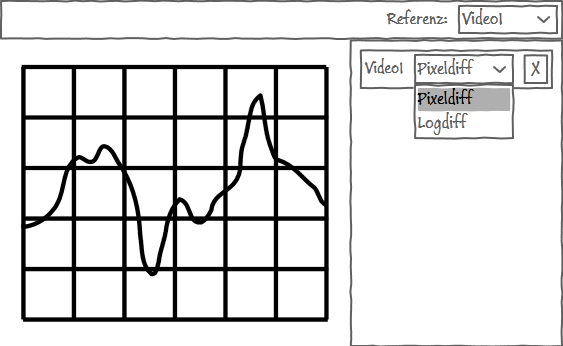
\includegraphics[scale=0.8]{resources/diagram-screen.png}
	\caption{Diagrammansicht eines Outputs}
\end{figure}

\section{Testfälle}

\textbf{Folgende Funktionssequenzen sind zu überprüfen:}
\begin{itemize}
	\item\textbf{/T10/} Pipeline-Konstruktion
		\begin{itemize}
			\item Der Benutzer startet das Programm.
			\item Der Benutzer wählt "Neue Pipline erstellen".
			\item Der Benutzer erzeugt jede Art von Knoten mindestens einmal indem er jeden Knoten per "Drag-and-Drop" aus einer am unteren Bildschirmrand
				angebrachten Leiste erzeugt.
			\item Der Benutzer verbindet die erstellten Knoten miteinader, indem er Kanten zwischen den Aus- und Eingängen der Knoten erstellt.
		\end{itemize}
	\item\textbf{/T20/} Manipulation einer Pipeline
		\begin{itemize}
			\item Der Benutzer startet das Programm und erstellet eine beliebige Pipeline mit mindestens 2 Knoten, davon mindestens ein Manipulationsknoten mit Optionen 
				und mindestens einer Kante.
			\item Der Benutzer bewegt mindestens einen gesetzte Knoten innerhalb der Pipeline per "Drag-and-Drop".
			\item Der Benutzer verändert das Ziel mindestens einer gesetzten Kante per "Drag-and-Drop".
			\item Der Benutzer löscht mindestens eine Kante.
			\item Der Benutzer verändert mindestens eine Einstellung eines Manipulationsknotens.
			\item Der Benutzer löscht mindestens einen Knoten.
		\end{itemize}
	\item\textbf{/T30/} Sicherung einer Pipeline
		\begin{itemize}
			\item Der Benutzer startet das Programm und erstellet eine beliebige Pipeline.
			\item Der Benutzer speichert die Pipeline.
			\item Der Benutzer wählt "Neue Pipeline erstellen".
			\item Der Benutzer läd die gesicherte Pipeline.
		\end{itemize}
\newpage
	\item\textbf{/T40/} Videoverarbeitung
		\begin{itemize}
			\item Der Benutzer startet das Programm und erstellet eine beliebige, zusammenhängende, zyklenfreie Pipeline mit mindestens einem Eingabe-, Wiedergabe- sowie 
				Manipulationsknoten mit Optionen.
			\item Der Benutzer ändert die Quelle eines EingabeKnotens.
			\item Der Benutzer öffnet den Wiedergabeknoten, and beginnt das Video abzuspielen.
			\item Der Benutzer ändert mindestens eine Option eines Manipulationsknotens, während das Video abspielt.
			\item Der Benutzer ändert die Abspielgeschwindigkeit des Videos.
			\item Der Benutzer pausiert die Videowiedergabe.
			\item Der Benutzer setzt die Wiedergabe fort.
			\item Der Benutzer setzt die Videowiedergabe zurück.
			\item Der Benutzer speichert das manipulierte Video als YUV-Datei.
		\end{itemize}
	\item\textbf{/T50/} Videoanalyse
		\begin{itemize}
			\item Der Benutzer startet das Programm und erstellet eine beliebige, zusammenhängende, zyklenfreie Pipeline mit mindestens einem Eingabe-, Überlagerungs- sowie 
				Diagrammknoten.
			\item Der Benutzer deaktiviert den Diagrammknoten.
			\item Der Benutzer öffnet den Überlagerungsknoten.
			\item Der Benutzer beginnt die Videowiedergabe.
			\item Der Benutzer fügt eine Überlagerungsoption hinzu, während das Video abspielt.
			\item Der Benutzer entfernt die hinzugefügte Überlagerungsoption.
			\item Der Benutzer setzt die Videowiedergabe zurück und schließt den Überlagerungsknoten.
			\item Der Benutzer reaktiviert den Dieagrammknoten und öffnet diesen.
			\item Der Benutzer wählt ein Referenzvideo aus und fügt einen Analysegraphen hinzu.
			\item Der Benutzer startet erneut die Videowiedergabe.
			\item Der Benutzer ändert den Typ des Analysegraphen.
			\item Der Benutzer löscht den Analysegraphen.
		\end{itemize}
\end{itemize}

\newpage

\textbf{Folgende Datenkonsistenzen sind einzuhalten:}
\begin{itemize}
	\item\textbf{/T100/} Ergebnislose Wiedergabe verhindern. ~\\
		Wenn der Benutzer keinen Endknoten geöffnet hat, ist die Videowiedergabe nicht anwählbar.
	\item\textbf{/T110/} Verarbeitung ohne Eingabe verhindern. ~\\
		Falls ein Eingabeknoten ohne gültige Videoquelle mit der Pipeline verbunden ist, ist weder die Videowiedergabe, noch das Speichern von Videos als YUF-Datei möglich.
	\item\textbf{/T120/} Strukturbrüche während der Wiedergabe verhindern ~\\
		Während der Videowiedergabe kann der Benutzer die Pipelinestruktur nicht verändern.
	\item\textbf{/T130/} Inkonsistenz eines gespeicherten Videos verhindern ~\\
		Während dem Speichern eines Videos als YUF-Datei kann der Benutzer keinerlei Änderungen an der Pipeline vornehmen.
\end{itemize}

\section{Qualitätsbestimmung}

%\begin{table}[htbp]
%\begin{tabularx}{1.2\textwidth}{|l|X|X|X|X|}
\begin{tabular}{@{\extracolsep{\fill}} |l|c|c|c|c|}
\hline
Produktqualität &  Sehr gut & Gut & Normal & Nicht relevant \\ \hline
\textbf{Funktionalität} &  &  &  &  \\ \hline
Angemessenheit  &  & X &  &  \\ \hline
Richtigkeit  &  & X &  &  \\ \hline
Interoperabilität  &  &  &  & X \\ \hline
Ordnungsmäßigkeit  &  &  & X &  \\ \hline
Sicherheit  &  &  &  & X \\ \hline
\textbf{Zuverlässigkeit} &  &  &  &  \\ \hline
Reife  &  &  & X &  \\ \hline
Fehlertoleranz  &  &  & X &  \\ \hline
Wiederherstellbarkeit  &  &  & X &  \\ \hline
\textbf{Benutzbarkeit} &  &  &  &  \\ \hline
Verständlichkeit  & X &  &  &  \\ \hline
Erlernbarkeit  & X &  &  &  \\ \hline
Bedienbarkeit & X &  &  &  \\ \hline
\textbf{Effizienz} &  &  &  &  \\ \hline
Zeitverhalten  &  & X &  &  \\ \hline
Verbrauchsverhalten  &  &  & X &  \\ \hline
\textbf{Änderbarkeit} &  &  &  &  \\ \hline
Analysierbarkeit &  & X &  &  \\ \hline
Modifizierbarkeit & X &  &  &  \\ \hline
Stabilität &  & X &  &  \\ \hline
Prüfbarkeit &  & X &  &  \\ \hline
\textbf{Übertragbarkeit} &  &  &  &  \\ \hline
Anpassbarkeit &  &  &  & X \\ \hline
Installierbarkeit &  &  & X &  \\ \hline
Konformität  &  &  & X &  \\ \hline
Austauschbarkeit  &  &  &  & X \\ \hline
\end{tabular}
%\end{tabularx}
%\end{table}
%\bigskip
\paragraph{}
Es wird Wert auf die Benutzbarkeit und Modifizierbarkeit gelegt sowie auf die Angemessenheit und Richtigkeit der Funktionalität.

\section{Glossar}

\begin{itemize}
    \item Computer - Transistorarray
\end{itemize}



\end{document}
